\def\QRCODE{MASTER_mispa_TUT.IMG.shape_from_focus_pythonqrcode.png}
\def\QRPAGE{http://www.iptutorials.science/tree/master/MASTER_mispa/TUT.IMG.shape_from_focus/python}
\pcorrectionsection{Python correction}

\begin{python}
import numpy as np
import matplotlib.pyplot as plt
from mpl_toolkits.mplot3d import Axes3D
from skimage import io
from scipy import ndimage
from matplotlib import cm
\end{python}

\subsection{Main function}
This code is used as the main function to perform shape-from-focus reconstruction. 

\begin{python}
volumes = ['cornee', 'vickers'];
for v in volumes:
    I = io.imread('volume_'+v+'.tif');
    I = I.astype('float');
    F = np.zeros(I.shape)
    N = 11;
    
    myfunctions = [variance, tenengrad, sml];
    for f in myfunctions:
        for i,im in enumerate(I):
            F[i] = f(im, N);
            
        # Evaluates altitudes and textures
        Z = np.argmax(F, axis=0);
        Z = ndimage.minimum_filter(Z, size=5);
        T = extractTexture(I, Z);
\end{python}

The extraction of the texture from the altitudes (indexes) in the stack of images is performed by the following function:
\begin{python}
def extractTexture(I, Z):
    """
    Extract texture from stack of images I, where Z is the index (altitude)
    I: stack of images, of shape (n, X, Y)
    Z: index of SFF maximum (of shape (X,Y)), values are between 0 and n-1
    returns basically I[Z(i,j], i, j)] for all (i,j)
    """
    m,n = I.shape[1:]
    ii,jj = np.ogrid[:m,:n]
    T = I[Z, ii, jj];
    return T;
\end{python}


\subsection{Sum of Modified Laplacian}
Results are illustrated in Fig.\ref{fig:sff:python:sml}.

\begin{python}
def sml(I, N):
    """
    SFF measure, SUM of modified Laplacian
    I: image
    N: neiborhood size
    returns: SFF measure for each pixel
    """
    h=np.array([[-1, 2, -1]]);
    ML=np.abs(ndimage.convolve(I,h))+np.abs(ndimage.convolve(I,np.transpose(h)));
    S=ndimage.uniform_filter(ML, N);
    return S;
\end{python}

\begin{figure}[H]
 \centering\caption{Texture and altitude reconstruction with the SML method.}%
 \hfill\subfloat[Texture.]{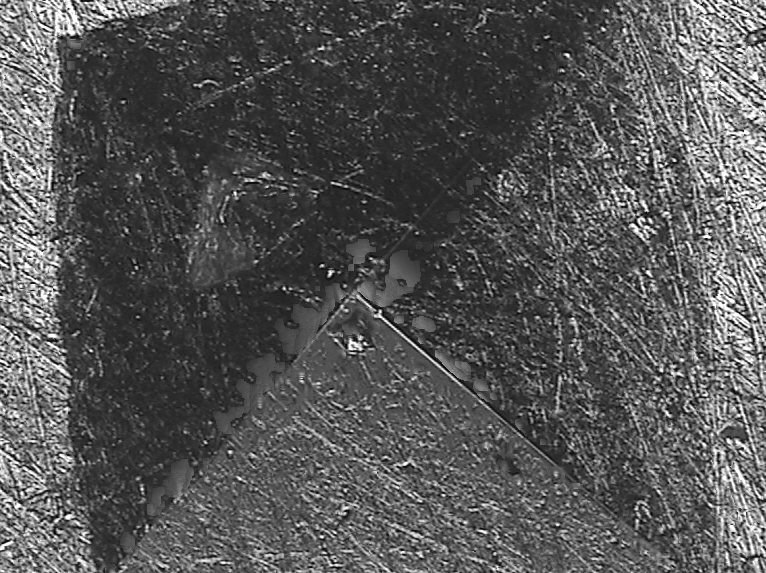
\includegraphics[width=.4\linewidth]{sml_vickers_texture.png}}\hfill\hfill
 \subfloat[Altitudes.]{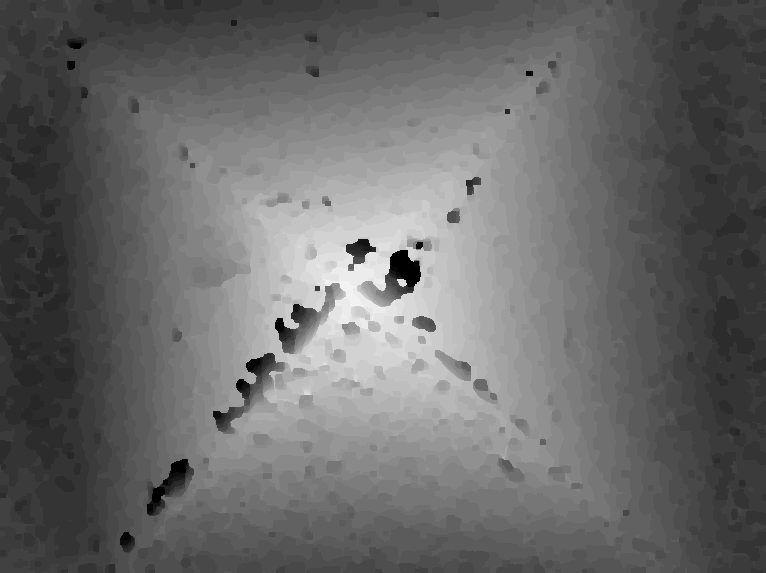
\includegraphics[width=.4\linewidth]{sml_vickers_altitudes.png}}\hfill\null

\vspace*{-5pt}

 \hfill\subfloat[Texture.]{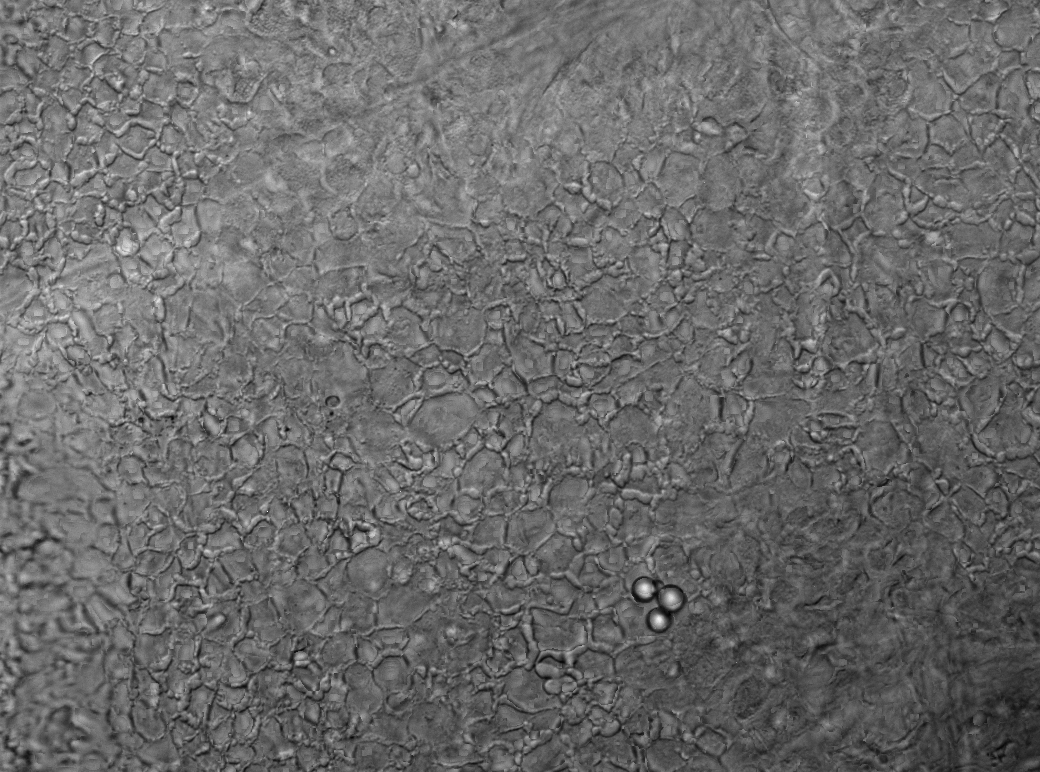
\includegraphics[width=.4\linewidth]{sml_cornee_texture.png}}\hfill\hfill
 \subfloat[Altitudes.]{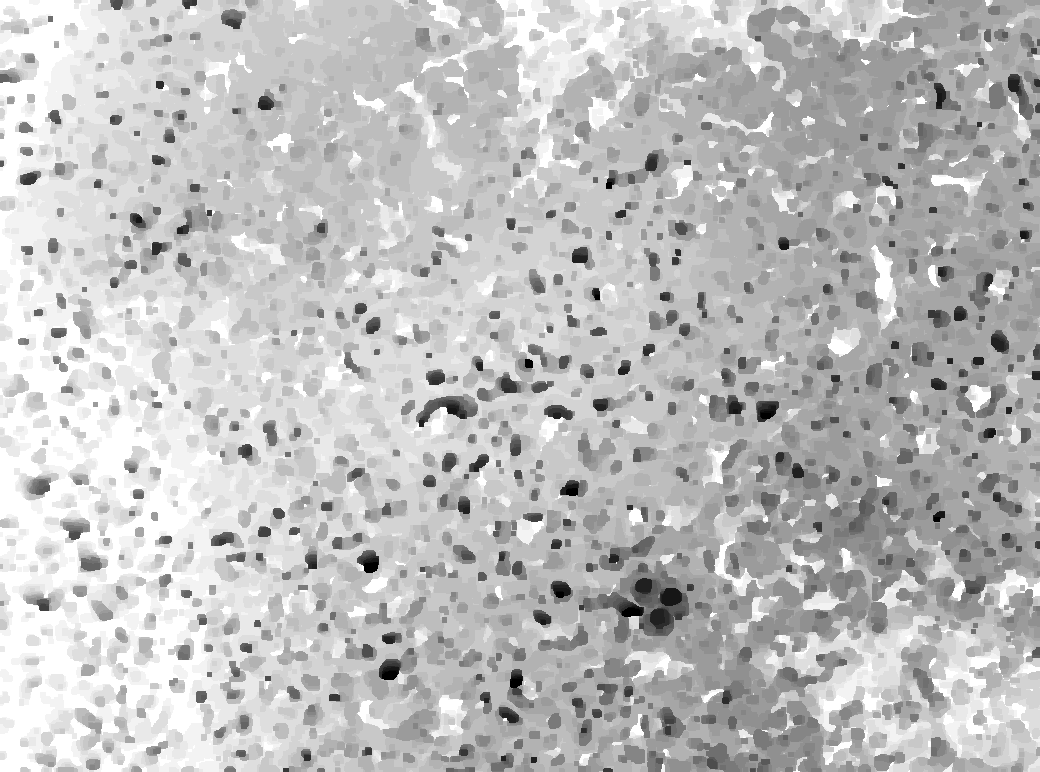
\includegraphics[width=.4\linewidth]{sml_cornee_altitudes.png}}\hfill\null%
 \vspace*{-5pt}%
 \label{fig:sff:python:sml}% 
\end{figure}


\subsection{Variance}
The focus measure based on the variance i a really simple method that works in most cases, see Fig.\ref{fig:sff:python:variance}.



\begin{python}
def variance(I, N):
    """
    SFF measure
    I: image
    N: neighborhood size
    returns: SFF measure for each pixel, results is the same shape as I
    """
    M = ndimage.uniform_filter(I, N);
    D2 = (I - M) ** 2;
    V = ndimage.uniform_filter(D2, N);
    return V;
\end{python}

\begin{figure}[htbp]
	\centering\caption{Texture and altitude reconstruction with the variance method.}%
	\hfill\subfloat[Texture.]{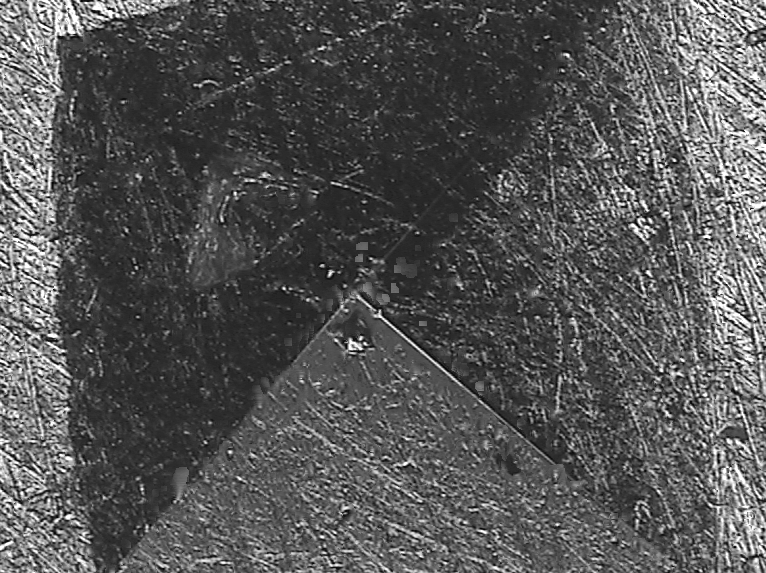
\includegraphics[width=.35\linewidth]{variance_vickers_texture.png}}\hfill\hfill
	\subfloat[Altitudes.]{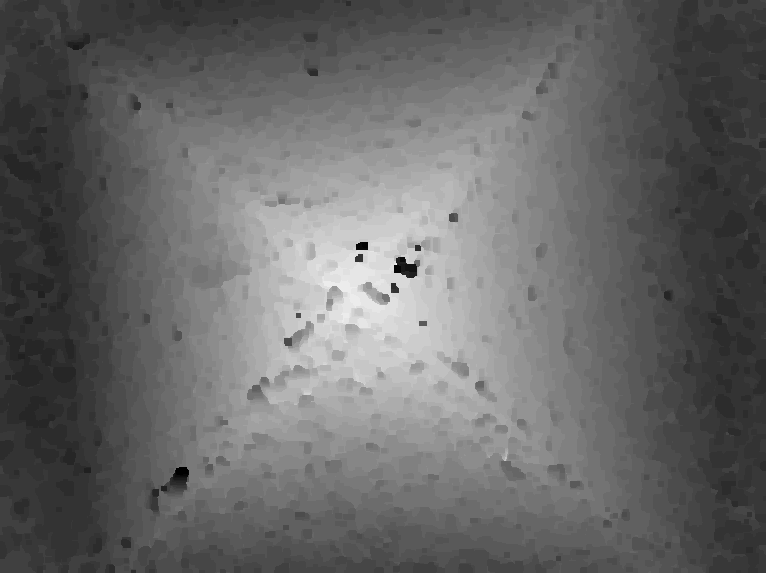
\includegraphics[width=.35\linewidth]{variance_vickers_altitudes.png}}\hfill\null
	
	\hfill\subfloat[Texture.]{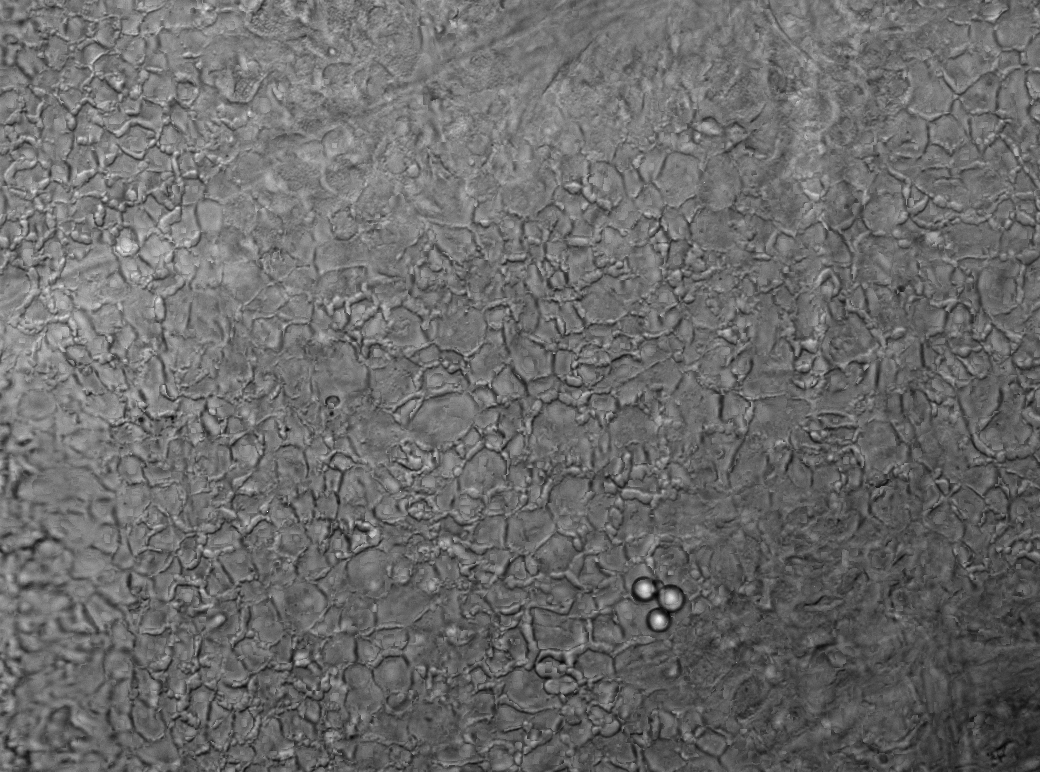
\includegraphics[width=.35\linewidth]{variance_cornee_texture.png}}\hfill\hfill
	\subfloat[Altitudes.]{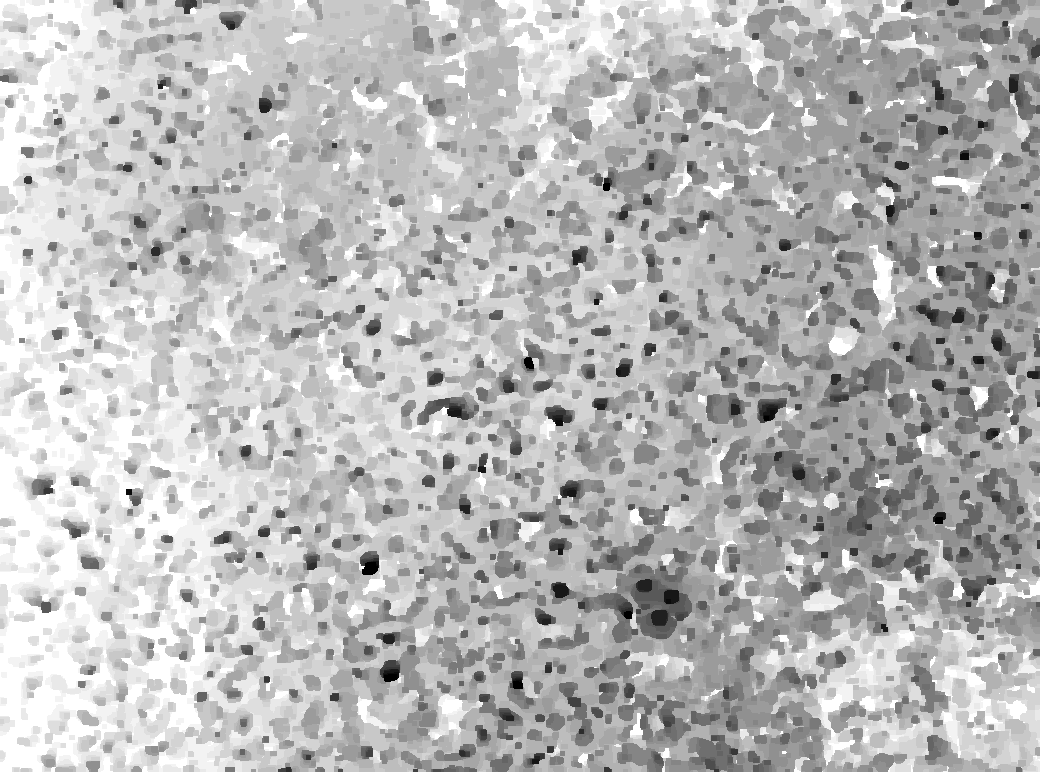
\includegraphics[width=.35\linewidth]{variance_cornee_altitudes.png}}\hfill\null%
	\label{fig:sff:python:variance}%
	\vspace*{-8pt}%
\end{figure}

\vspace*{-15pt}

\subsection{Tenengrad}
The tenengrad method is base on a Sobel filter, see Fig.\ref{fig:sff:python:tenengrad}.

\begin{python}
def tenengrad(I, N):
    """
    SFF measure, Tenengrad method
    I: image
    N: neighborhood size
    returns: SFF measure for each pixel, results is the same shape as I
    """
    Sx = ndimage.sobel(I, axis=0);
    Sy = ndimage.sobel(I, axis=1);
    S = np.hypot(Sx, Sy);
    T = ndimage.uniform_filter(S, N);
    return T;
\end{python}

\vspace*{-3pt}

\subsection{Variance of Tenengrad}
The variance of Tenengrad is an improvement of the Tenengrad method, see Fig.\ref{fig:sff:python:variancetenengrad}.

\begin{python}
def varianceTenengrad(I, N):
    """
    SFF measure, variance of Tenengrad
    I: image
    N: neiborhood size
    returns: SFF measure for each pixel
    """
    Sx = ndimage.sobel(I, axis=0);
    Sy = ndimage.sobel(I, axis=1);
    S = np.hypot(Sx, Sy);
    vt = variance(S, N);
    return vt;
\end{python}

\begin{figure}[htbp]
	\centering\caption{Texture and altitude reconstruction with the SML method.}%
	\hfill\subfloat[Texture.]{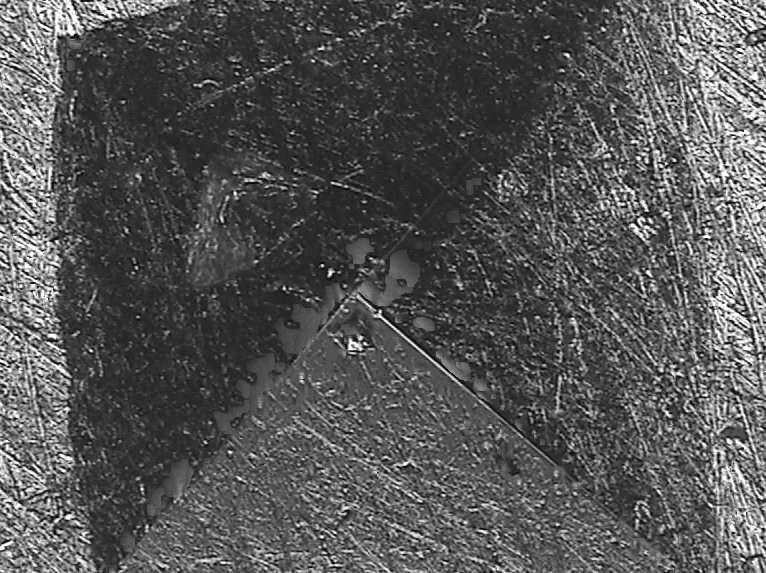
\includegraphics[width=.35\linewidth]{tenengrad_vickers_texture.png}}\hfill\hfill
	\subfloat[Altitudes.]{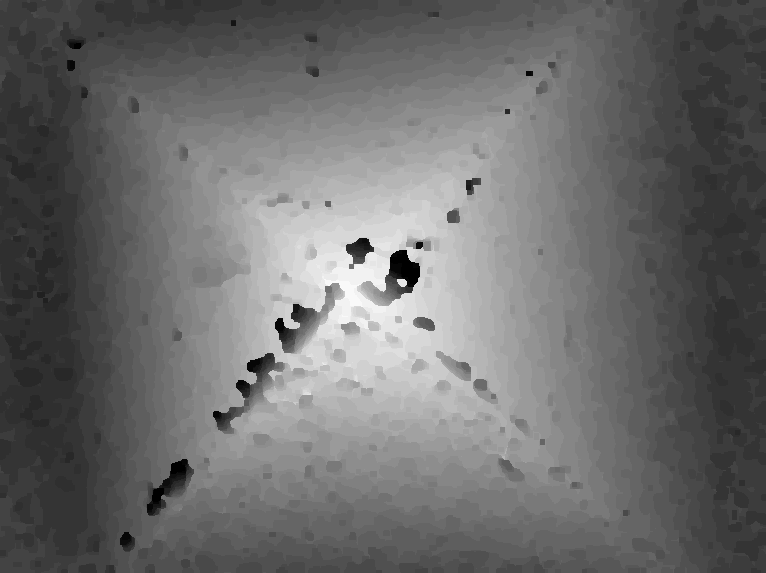
\includegraphics[width=.35\linewidth]{tenengrad_vickers_altitudes.png}}\hfill\null
	
	\hfill\subfloat[Texture.]{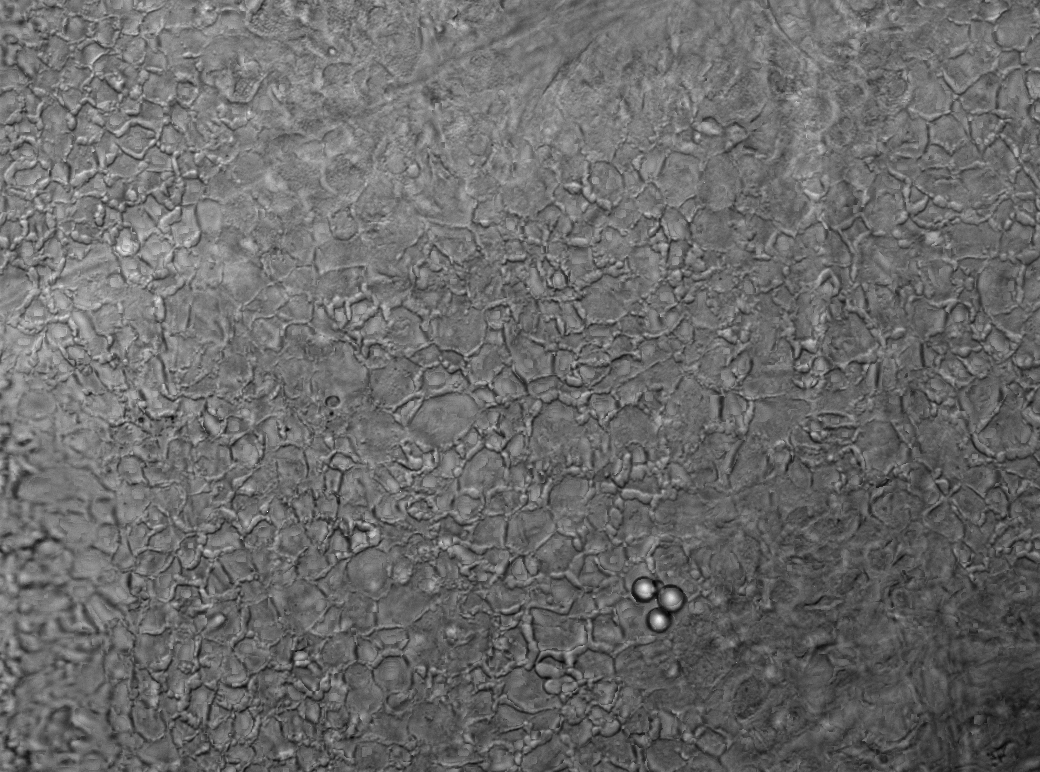
\includegraphics[width=.35\linewidth]{tenengrad_cornee_texture.png}}\hfill\hfill
	\subfloat[Altitudes.]{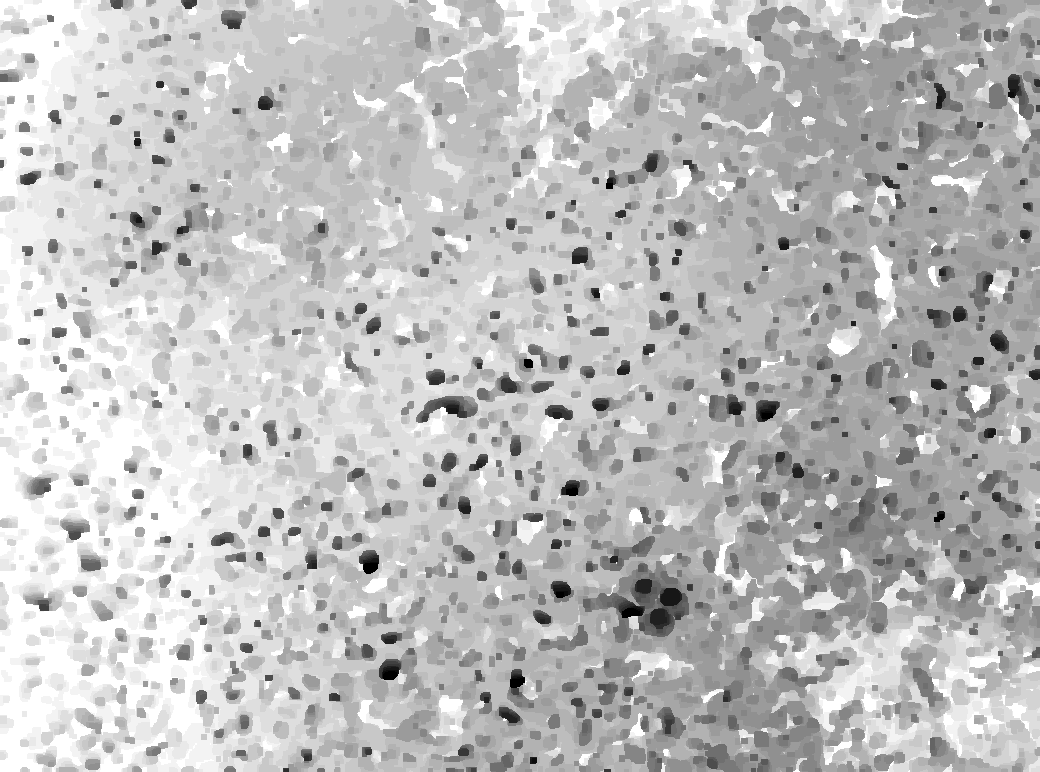
\includegraphics[width=.35\linewidth]{tenengrad_cornee_altitudes.png}}\hfill\null\label{fig:sff:python:tenengrad}%	
\end{figure}

\begin{figure}[htbp]
 \centering\caption{Texture and altitude reconstruction with the variance of Tenengrad method.}%
 \hfill\subfloat[Texture.]{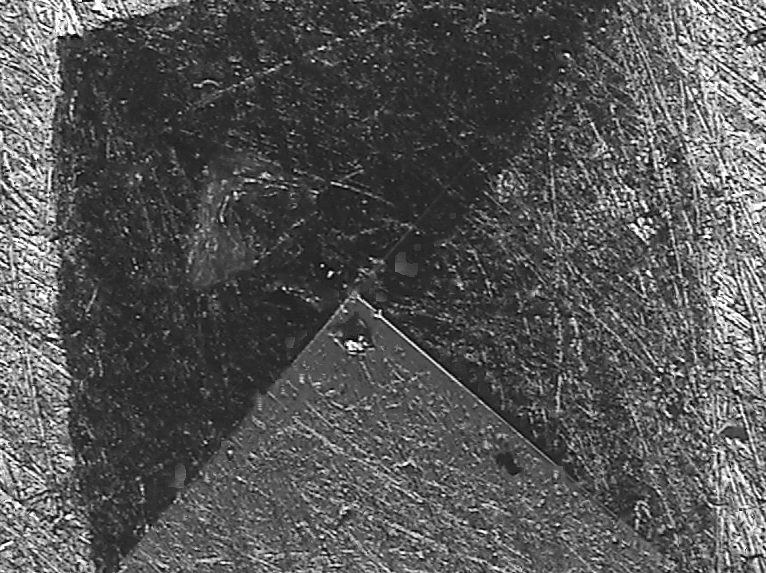
\includegraphics[width=.35\linewidth]{varianceTenengrad_vickers_texture.png}}\hfill\hfill
 \subfloat[Altitudes.]{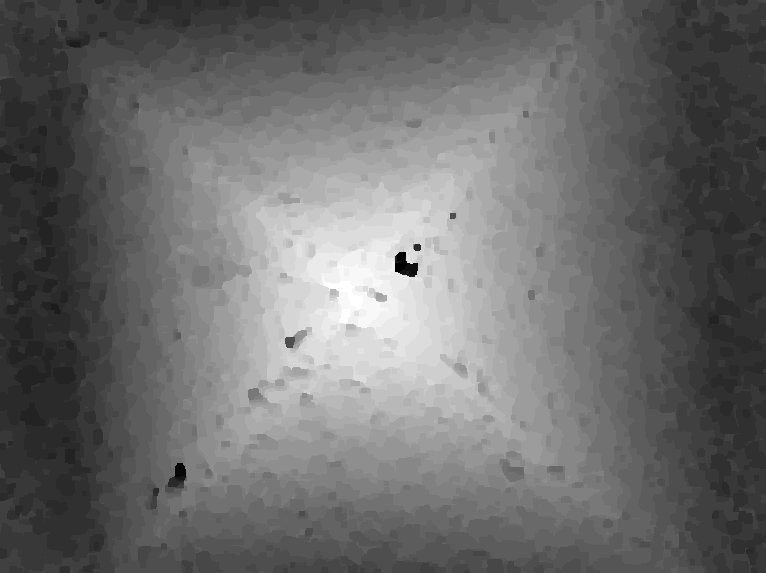
\includegraphics[width=.35\linewidth]{varianceTenengrad_vickers_altitudes.png}}\hfill\null

 \hfill\subfloat[Texture.]{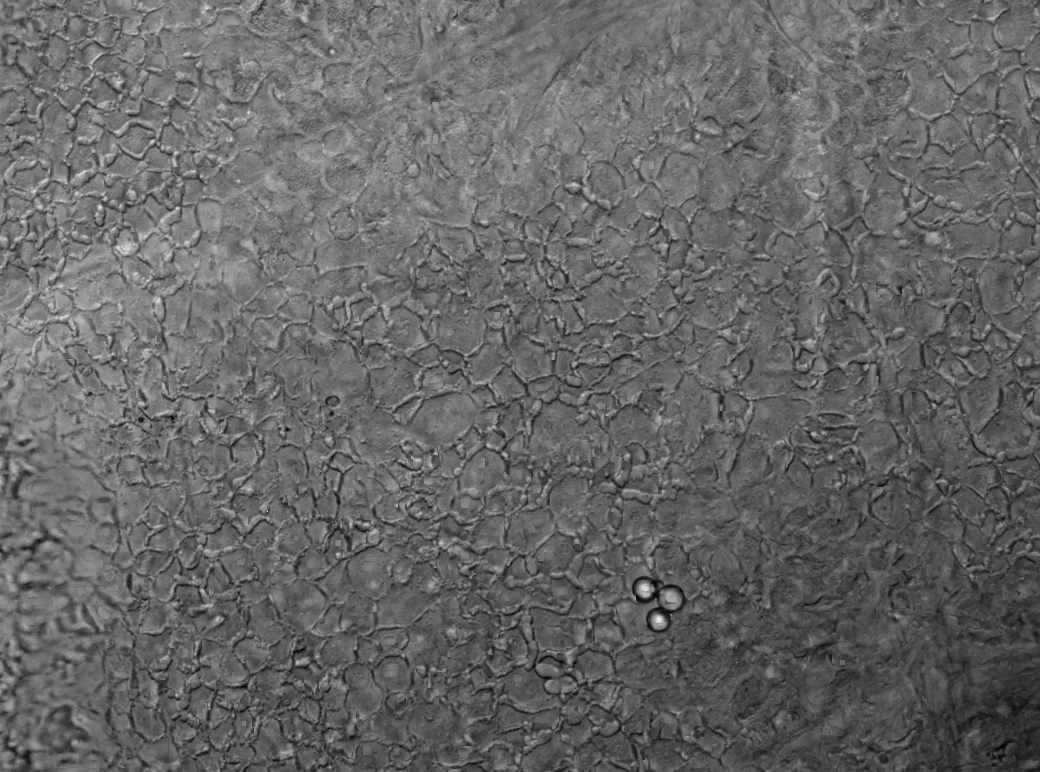
\includegraphics[width=.35\linewidth]{varianceTenengrad_cornee_texture.png}}\hfill\hfill
 \subfloat[Altitudes.]{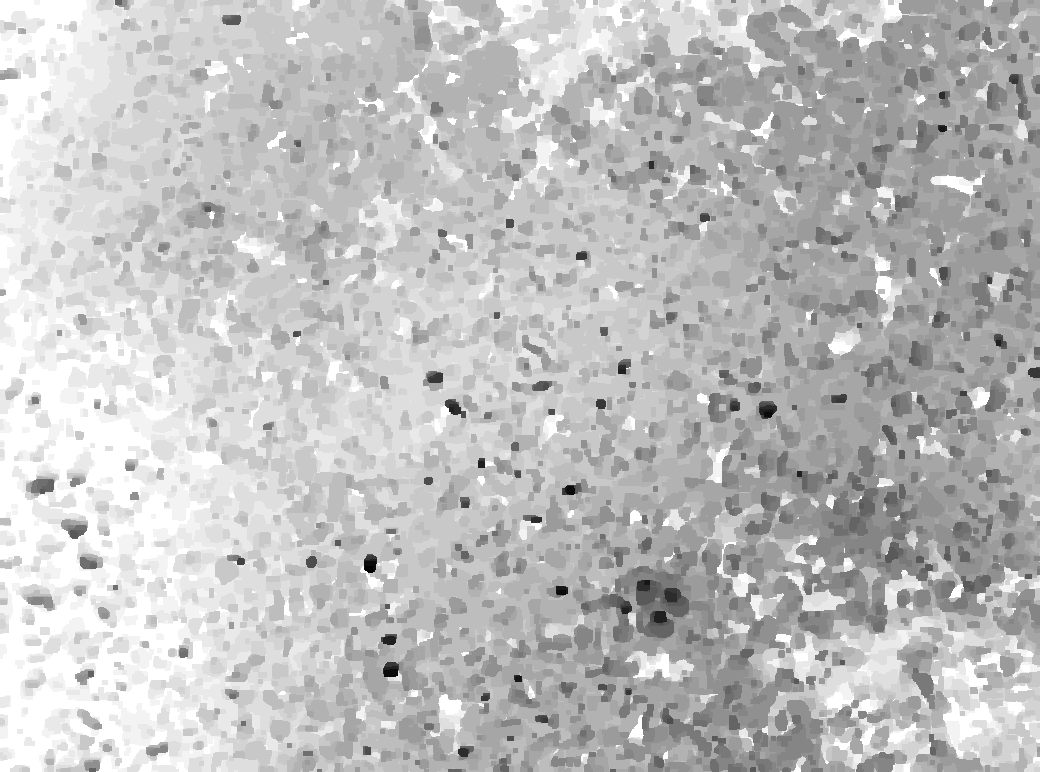
\includegraphics[width=.35\linewidth]{varianceTenengrad_cornee_altitudes.png}}\hfill\null%
 \label{fig:sff:python:variancetenengrad}%
\end{figure}
